\documentclass[aps,prc,twocolumn,floatfix,showpacs,a4paper,
nofootinbib,amsmath,amssymb]{revtex4}
%\documentclass[aps,preprint,showpacs,superscriptaddress,
%groupedaddress,amsmath,amssymb]{revtex4}
\usepackage{graphicx}
%\usepackage{dcolumn}
\usepackage{bm}
\usepackage{color}
\usepackage[colorlinks=true, allcolors=blue]{hyperref}
%\usepackage{subfig}
\usepackage{csquotes}
%\usepackage{diagbox}
%\usepackage{lipsum}
%\usepackage{setspace}
\newcommand{\be}{\begin{equation}}
\newcommand{\ee}{\end{equation}}
\newcommand{\ba}{\begin{eqnarray}}
\newcommand{\ea}{\end{eqnarray}}
\newcommand{\bd}{\begin{displaymath}}
\newcommand{\ed}{\end{displaymath}}
\newcommand{\bea}{\begin{eqnarray}}
\newcommand{\eea}{\end{eqnarray}}
\newcommand{\di}{{\rm d}}
\renewcommand{\vec}[1]{\mbox{\boldmath$#1$}}
%\DeclareMathOperator{\Artanh}{Artanh}
%\DeclareMathOperator{\Arsinh}{Arsinh}

\begin{document}

\title{A toy model for simulating $\alpha$ particle emissions in p + 11B reactions at $K_p=$10 MeV via Monte Carlo method}

\author{Angel Reina Ramirez, V. Magas}
\smallskip

%\affiliation{
%$^1$Departament de Fisica Quantica i Astrofisica,  
%Universitat\! de\! Barcelona,  Martí i Franquès 1, 08028 Barcelona, Spain\\
%$^2$Institut de Ciències del Cosmos,  
%Universitat\! de\! Barcelona,  Martí i Franquès 1, 08028 Barcelona, Spain\\
%$^3$Institute of Physics and Technology, University of Bergen,
%Allegaten 55, 5007 Bergen, Norway\\
%$^4$Frankfurt Institute for Advanced Studies (FIAS), Ruth-Moufang-Str. 1, 60438, %Frankfurt am Main, Germany\\
%$^5$Wigner Research Centre for Physics (RCP), XII. Konkoly Thege Miklós út 29-33, %Postbox 49, 1121 Budapest, Hungary\\
%$^6$Los Alamos National Laboratory, Los Alamos, 87545 New Mexico, USA
%}

%\acknowledgements

\begin{abstract}
We present a toy model for simulating $\alpha$ particle emissions in p$+$11B reactions at $K_p =$ 10 MeV via Monte Carlo method.  
Incident proton is accelerated along the z-axes by an oscillating electric field of frequency $\omega$, and its momentum is randomly generated at the moment of the collision. After collision, we get an $\alpha$ particle, emitted in z-direction, and an excited 8Be nucleus at rest, which breaks down in two $\alpha$ particles emitted in opposite direction. Pseudorandom number generator Mersenne twister engine algorithm is employed to randomly spawn the emisson angles of $\alpha$ particles. 
\end{abstract}
%\date{\today}
\maketitle
%\tableofcontents
%\pacs{25.75.-q, 24.70.+s, 47.32.Ef}

\section{Model description}



Incident proton is accelerated along the z-axes by an oscillating electric field of frequency $\omega$:
\begin{equation}
E_z = E_0cos(\omega t + \phi).
\end{equation}

From Newton's third law we get proton momentum:
\begin{equation}
F_z = e E_0cos(\omega t + \phi) = \frac{dp_z}{dt},
\end{equation}
\begin{equation}
p_z = \frac{eE_0}{\omega} sin(\omega t + \phi) = p_{z,max} sin(\omega t + \phi),
\end{equation}
where $p_{z,max} = \sqrt{2M_pK_p}$. Then $\omega t + \phi$ angle is randomly spawned at the time of the collision via the pseudorandom number generator: Mersenne twister engine algorithm. Incident proton collides with a 11B nucleus at rest to produce a 8Be excited nucleus at rest and an $\alpha$ particle moving in the same direction as incident proton. Thus, the polar angle $\theta_1$ at which this $\alpha$ particle is emitted is constrained to two values: $0$ and $\pi$, depending on if incident proton is moving forward or backward, respectively.



Later on, 8Be excited nucleus breaks down in two $\alpha$ particles moving in opposite direction. The angles $\theta_2$ and $\theta_3$ at which these two $\alpha$ particles are emitted are randonly spawned. Because of momentum conservation law, angle $\theta_3$ is constrained to
\be
\theta_3 = \pi - \theta_2,
\ee
so, actually, we just have to randomly generate $\theta_2$ angle. Similarly, the azimuthal angles are related by the following relation:
\be
\phi_3 = \pi + \phi_2.
\ee
Thus, in spherical coordinates the momentum of emitted $\alpha 1$ and $\alpha 2$ particles are 

\be
\vec{p_{\alpha2}} = p_{\alpha2}\left(sin(\theta_2)cos(\phi_2),sin(\theta_2)sin(\phi_2),cos(\theta_2)\right),
\ee
\be
\vec{p_{\alpha3}} = -p_{\alpha2}\left(sin(\theta_2)cos(\phi_2),sin(\theta_2)sin(\phi_2),cos(\theta_2)\right),
\ee
where $p_{\alpha 2}$ is obtained from the energy conservation law,
\be
M_p + \frac{p_p^2}{2M_p} + M_{11B} = M_{8Be}^* + M_{\alpha} + \frac{p_{\alpha1}^2}{2M_{\alpha}},
\ee

\be
M_{8Be}^* = M_{\alpha} + \frac{p_{\alpha2}^2}{2M_{\alpha}} + M_{\alpha} + \frac{p_{\alpha3}^2}{2M_{\alpha}},
\ee

\be
M_p + \frac{p_p^2}{2M_p} + M_{11B} = 3M_{\alpha} + \frac{p_{\alpha1}^2}{2M_{\alpha}} + \frac{p_{\alpha2}^2}{2M_{\alpha}} + \frac{p_{\alpha3}^2}{2M_{\alpha}},
\ee

\be
p_{\alpha1}^2 + p_{\alpha2}^2 + p_{\alpha3}^2 = 2M_{\alpha}\left(M_p + \frac{p_p^2}{2M_p} + M_{11B} - 3M_{\alpha}\right),
\ee

Because of $p_{\alpha2} = p_{\alpha3}$,

\be
p_{\alpha1}^2 + 2p_{\alpha2}^2 = 2M_{\alpha}\left(M_p + \frac{p_p^2}{2M_p} + M_{11B} - 3M_{\alpha}\right) = x.
\ee

\be
p_{\alpha2}^2 = (x - p_{\alpha1}^2) / 2.
\ee

So, we just have to randomly generate $p_{\alpha1}$, constrained to the interval [0,x].
 
In Fig. \ref{Reaction} is illustrated the collision betwen p and 11B nucleus, and its subsequent decay products.

\begin{figure}[h]
	\begin{center}
		\resizebox{0.98\columnwidth}{!}
		{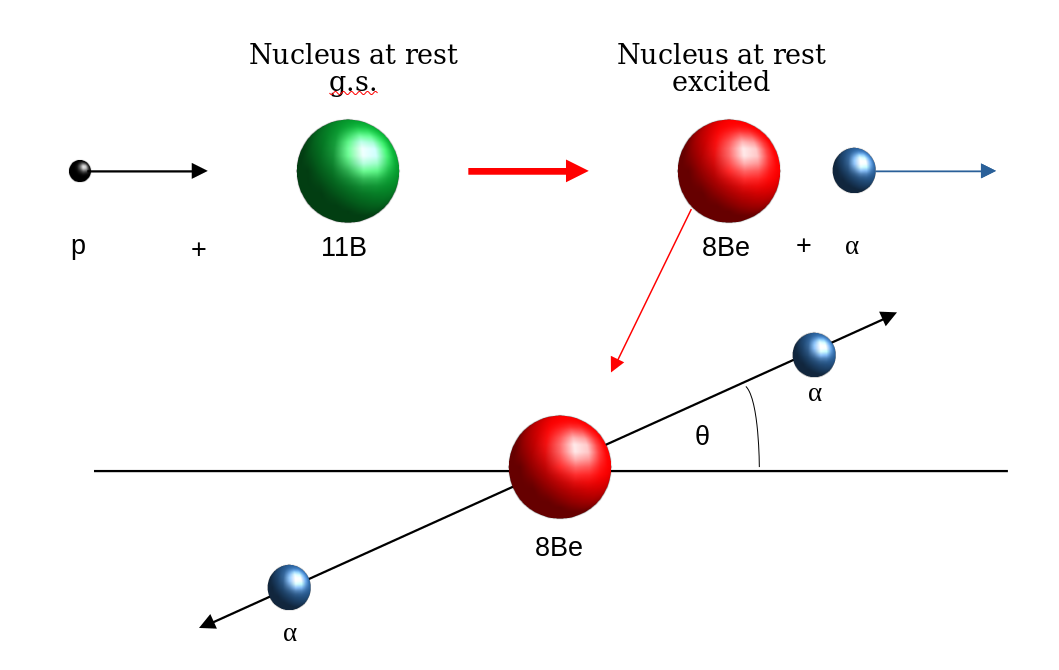
\includegraphics{reaction_scheme.png}}
		\caption{ (color online)
			Reaction scheme.
		}
		\label{Reaction}
	\end{center}
\end{figure} 



\section{Results}

We present the angular and the energy distributions of emitted $\alpha$ particles.

\subsection{Angular distribution of emitted $\alpha$ particles}
\begin{figure}[h!]
	\begin{center}
		\resizebox{0.98\columnwidth}{!}
		{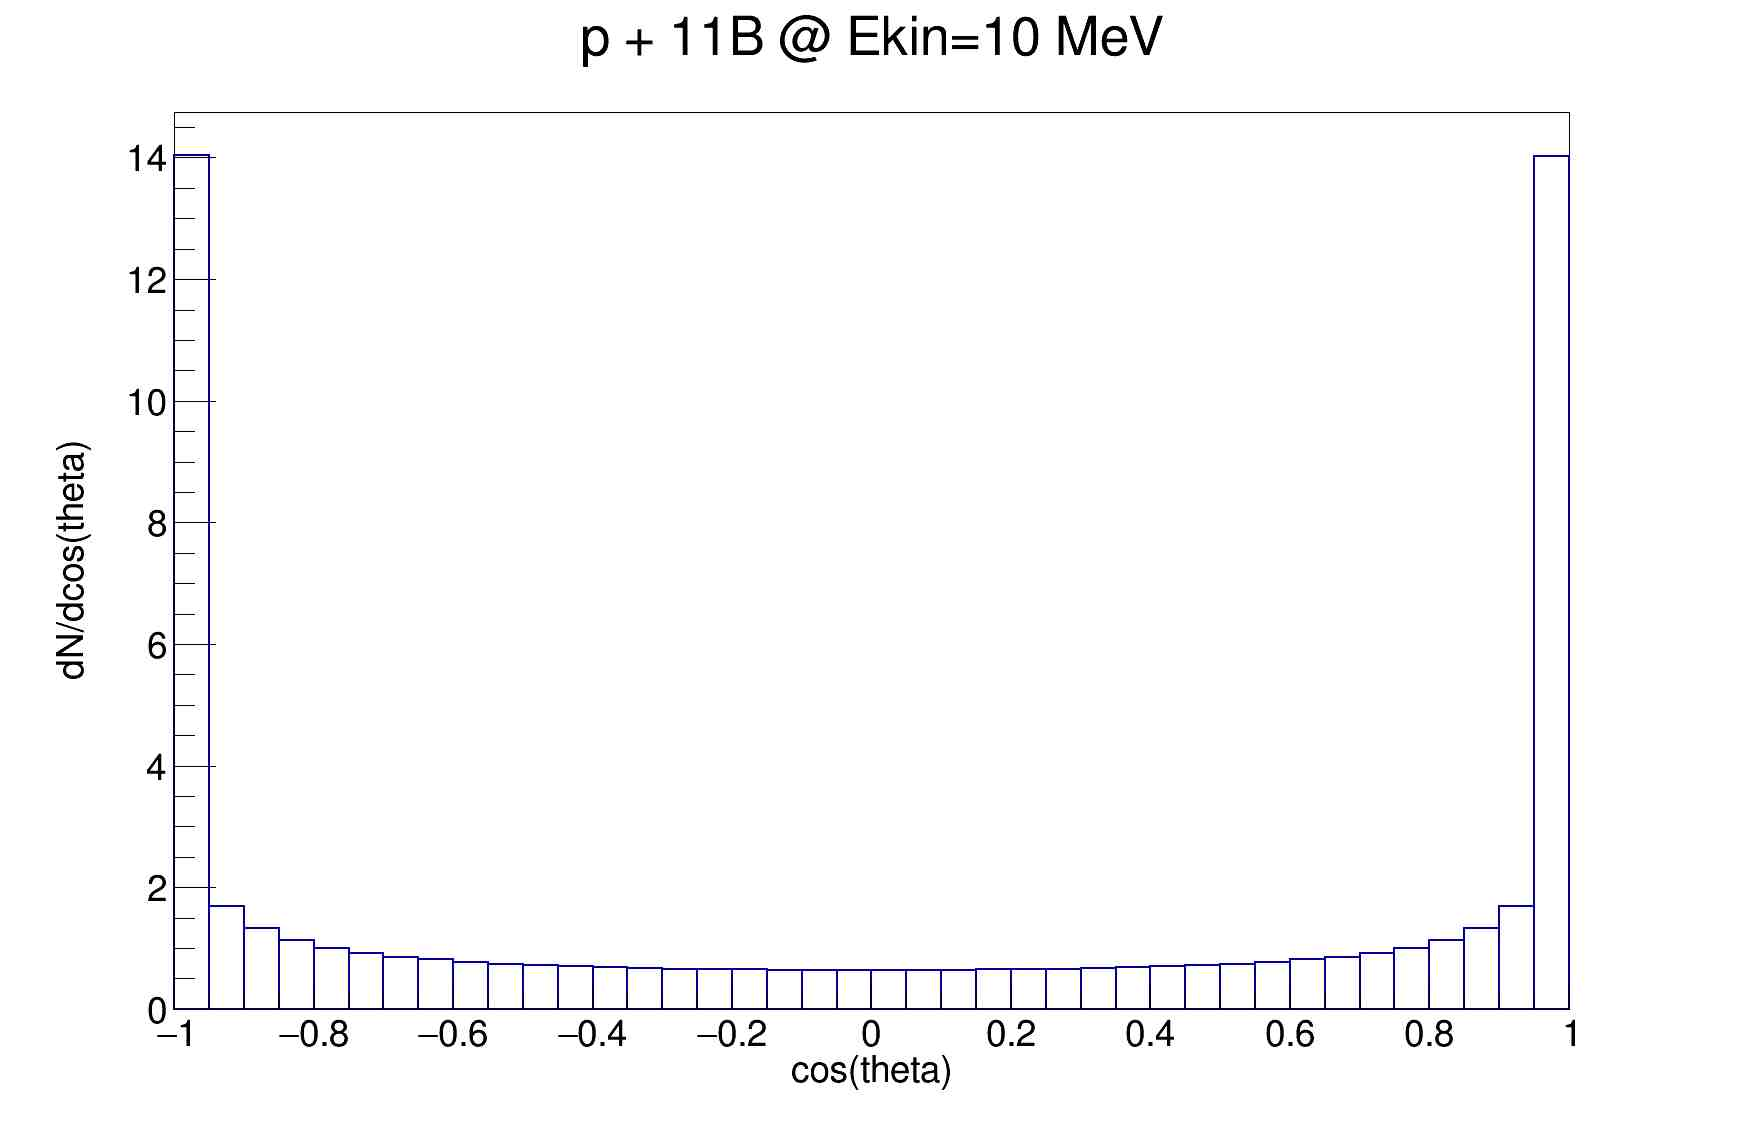
\includegraphics{dNdcostheta.jpg}}
		\caption{ (color online)
			Reaction scheme.
		}
		\label{Reaction}
	\end{center}
\end{figure} 

\subsection{Energy distribution of emitted $\alpha$ particles}
\begin{figure}[h!]
	\begin{center}
		\resizebox{0.98\columnwidth}{!}
		{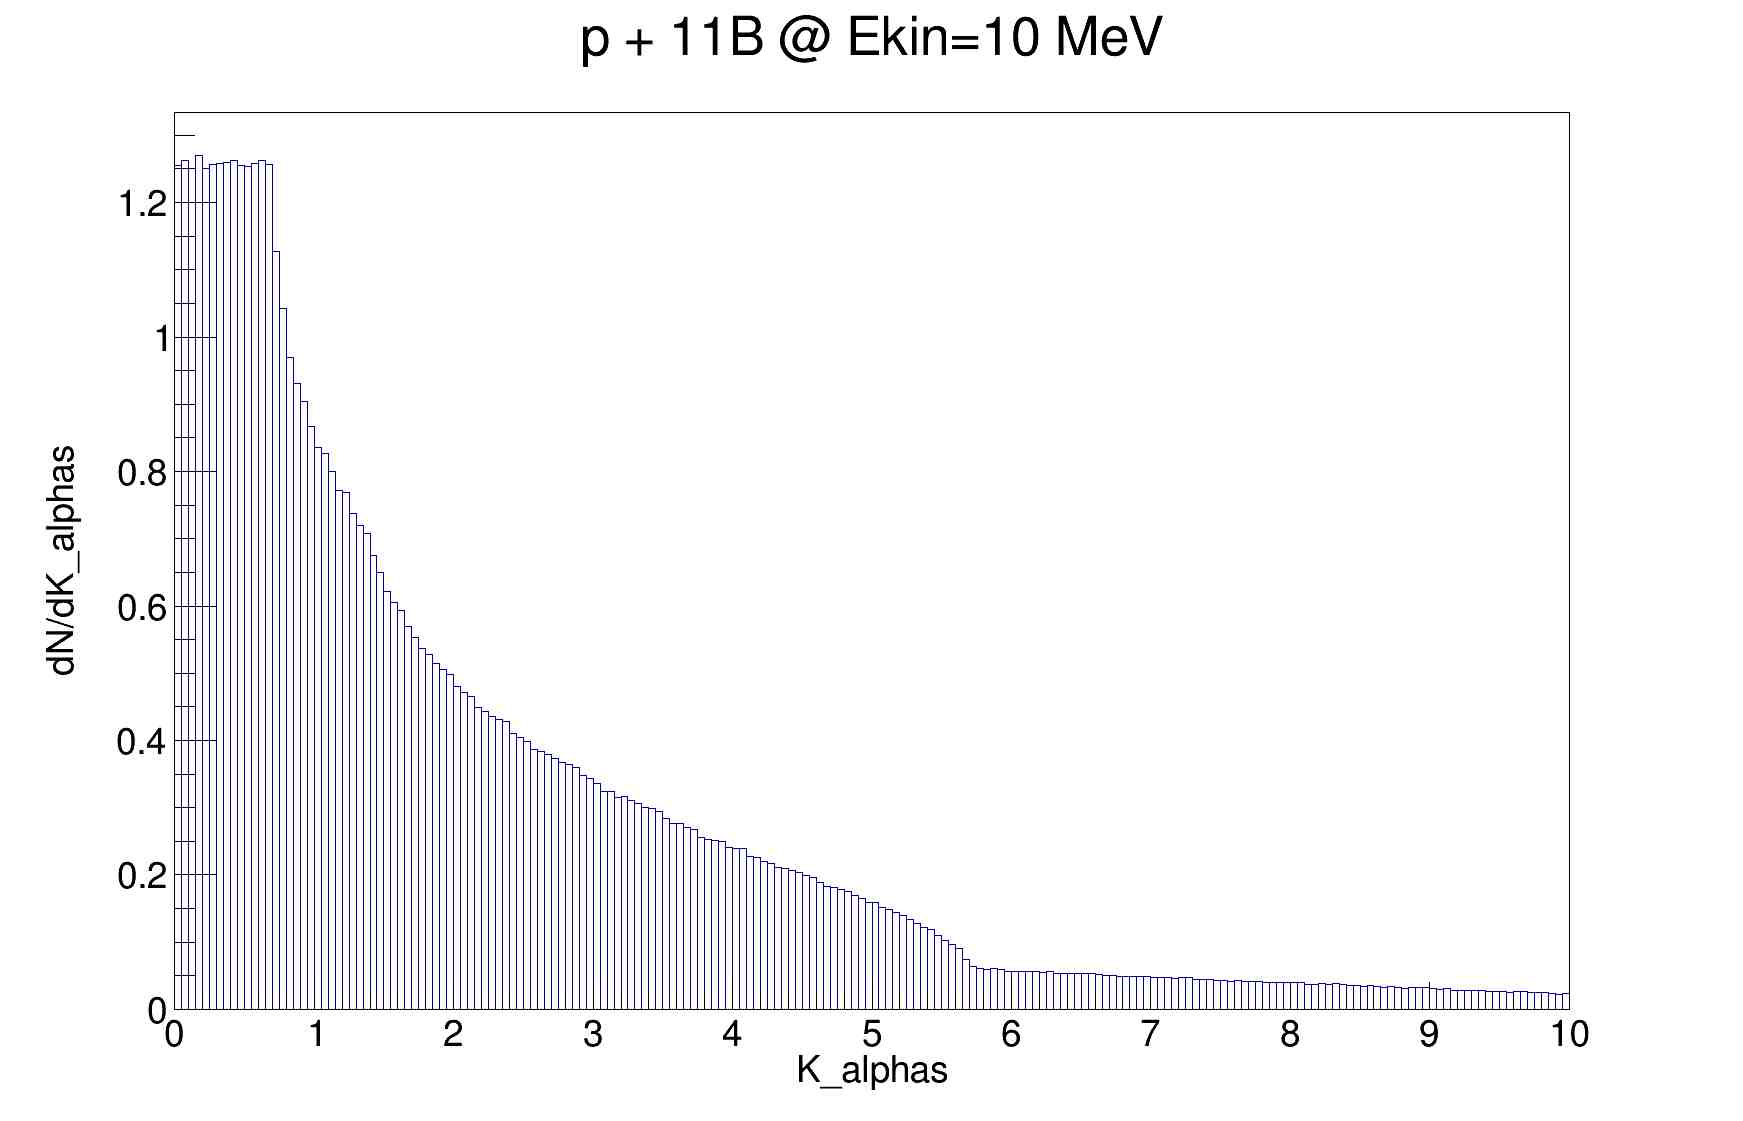
\includegraphics{dNdK.jpg}}
		\caption{ (color online)
			Reaction scheme.
		}
		\label{Reaction}
	\end{center}
\end{figure} 

\section{References}

\appendix{Appendix I}

\end{document}
